%%%%%% Discussion and conclusions
%While ... we think ....
We have presented a model for a more complex opinion than binary, single dimensional vectors. Furthermore, we compared three
common voting algorithms and showed sensible evidence in the suboptimality of plurality voting with respect to maximization
of each voter utility function, the happiness metric.
Furthermore, we have illustrated the effect of opinion transparency on elections in the complex opinion space;
namely that a candidate can ``fool''
their way into office by masking their opinion of select issues, thereby misleading voters.

\subsection{Voting strategies as search algorithms}
As a final note, we observe that in this fomulation of opinion as a $d$-length vector, voting algorithms function as search algorithms
that search the space of candidates and attempt to select the candidate that is the least distance in opinion from each voter
in the population.  This idea is illustrated in Figure~\ref{fig:plurality_vs_rc_anecdotal}. From the figure, we observe that both
ranked choice and approval based voting have determined more centrally located candidates with respect to the opinion space.
\begin{figure*}
%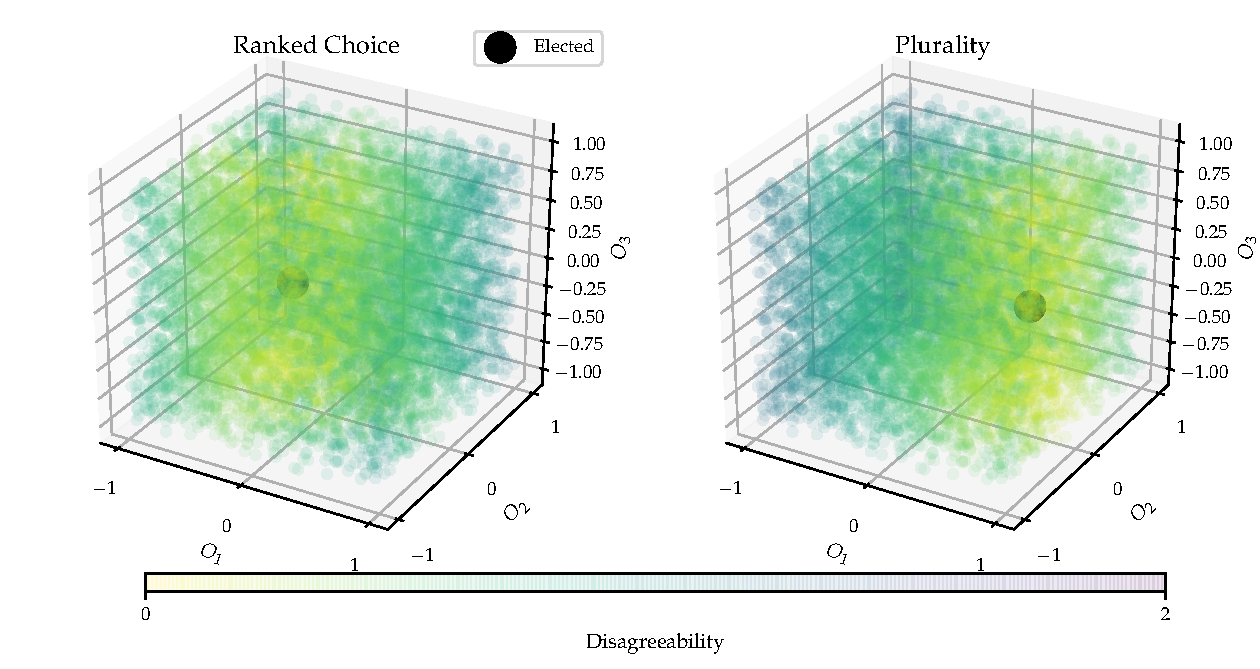
\includegraphics[width=1\textwidth]{../src/figs/uniform_opinions/rc-gen_anecdotal_comparison-3D.pdf}
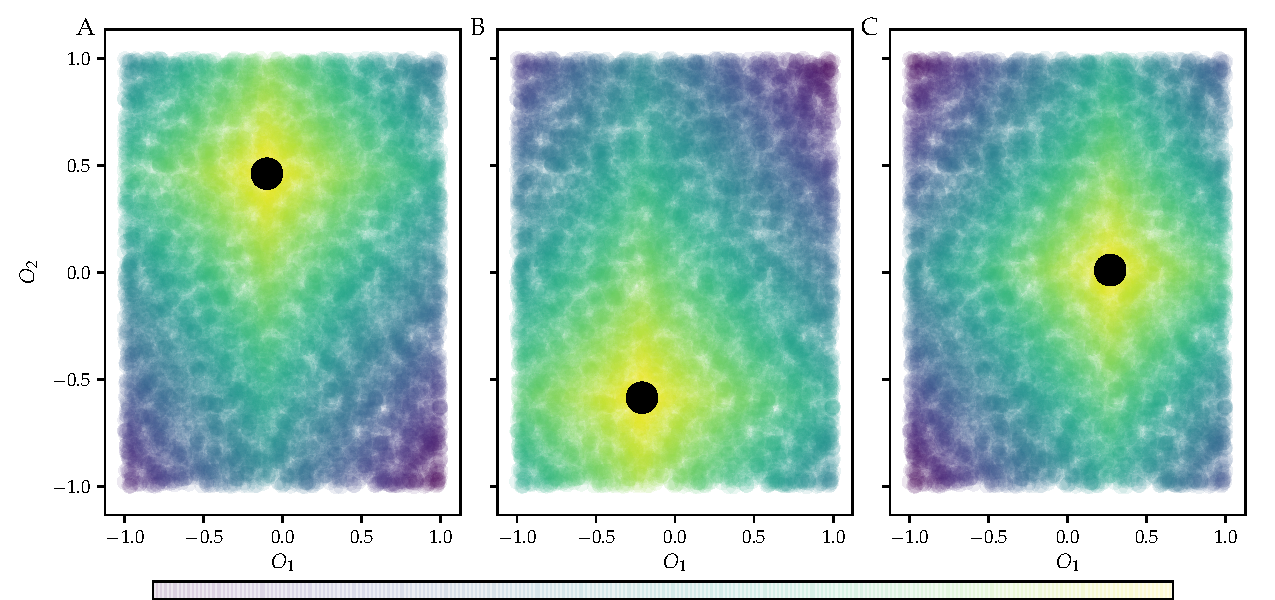
\includegraphics[width=1\textwidth]{figs/rc-gen_anecdotal_comparison-2D.pdf}\vspace{-3mm}
\caption{Elected candidate, marked with the black dots, in a 2-dimensional opinion space for a single sample population, comparing plurality \letter{A},
ranked-choice \letter{B}, and approval-based \letter{C} voting outcomes with average happiness ratings
$\bar{H_{\mathrm{plural}}}=0.7$, $\bar{H_{\mathrm{ranked}}}=0.72$, $\bar{H_{\mathrm{approve}}}=0.74$,
Each point is an opinion vector $(o_1, o_2)$ and its color is governed by the happiness of the voter with the winning candidate.}
\label{fig:plurality_vs_rc_anecdotal}
\end{figure*}
\section{Future Work}
In future work, we would like to further explore this model by informing our opinion vectors with data.
We think it could lead to even more interesting results if the opinions were drawn from different distributions for the different topic dimensions, possibly distributions representative of actual polling data on a variety of political topics.

For instance, the effect of the candidate opinion transparency would likely be much greater if all topics were not distributed the same in the opinion space, such that if one topic was heavily polarized and bi-modal and was masked by a candidate, it could lead to a much larger change in happiness outcome.

Much of the weakness of this study is in the purely stochastic set-up, where all seems to average out in the end.
But even though it was not heavily significant, the plurality voting system was the worst for overall happiness in every scenario run, and surprisingly approval voting, which is similarly simple came out ahead a couple times.

Furthermore, we would like to investigate the idea of utilizing a different metric for disagreeability. We belive that though our results are sound, the proposed metric function makes little use of its entire range as see in
Figures~\ref{fig:avghapp_by_transparency} and~\ref{fig:satisfaction_hists}. We would also like to further investigate the notion
of opinion transparency and trace its effect on the system.

Additionally, there are many more branches to expand this research. Incorporating the notion of no-show voters, contrarians,
and opinion-polarizing candidates.
